
\subsection{Data Dictionary Diagram}


\begin{figure}[H]
    \centering
    \caption{Data Dictionary Diagram 1}
    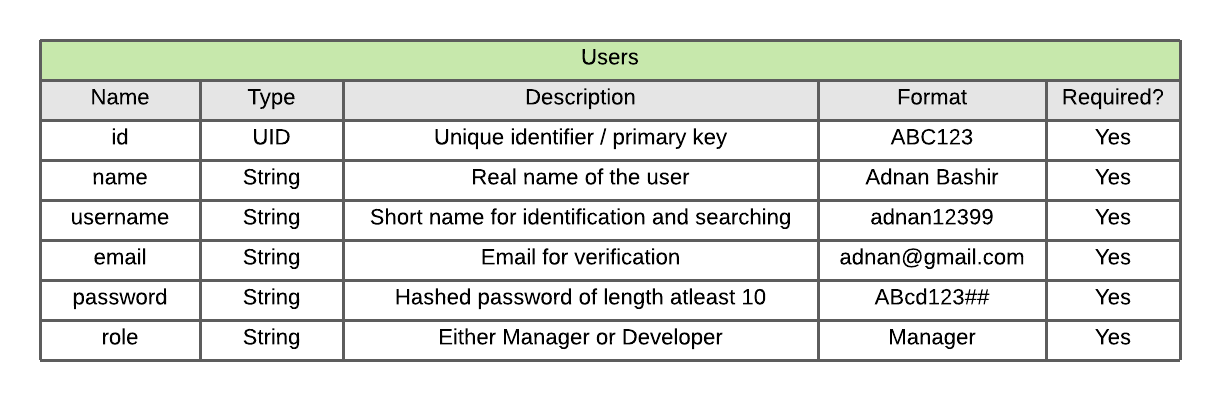
\includegraphics[scale=0.7]{./diagrams/data-dictionary/dd-1.png}
    \label{fig:dd-diag-1}

\end{figure}


\begin{figure}[H]
    \centering
    \caption{Data Dictionary Diagram 2}
    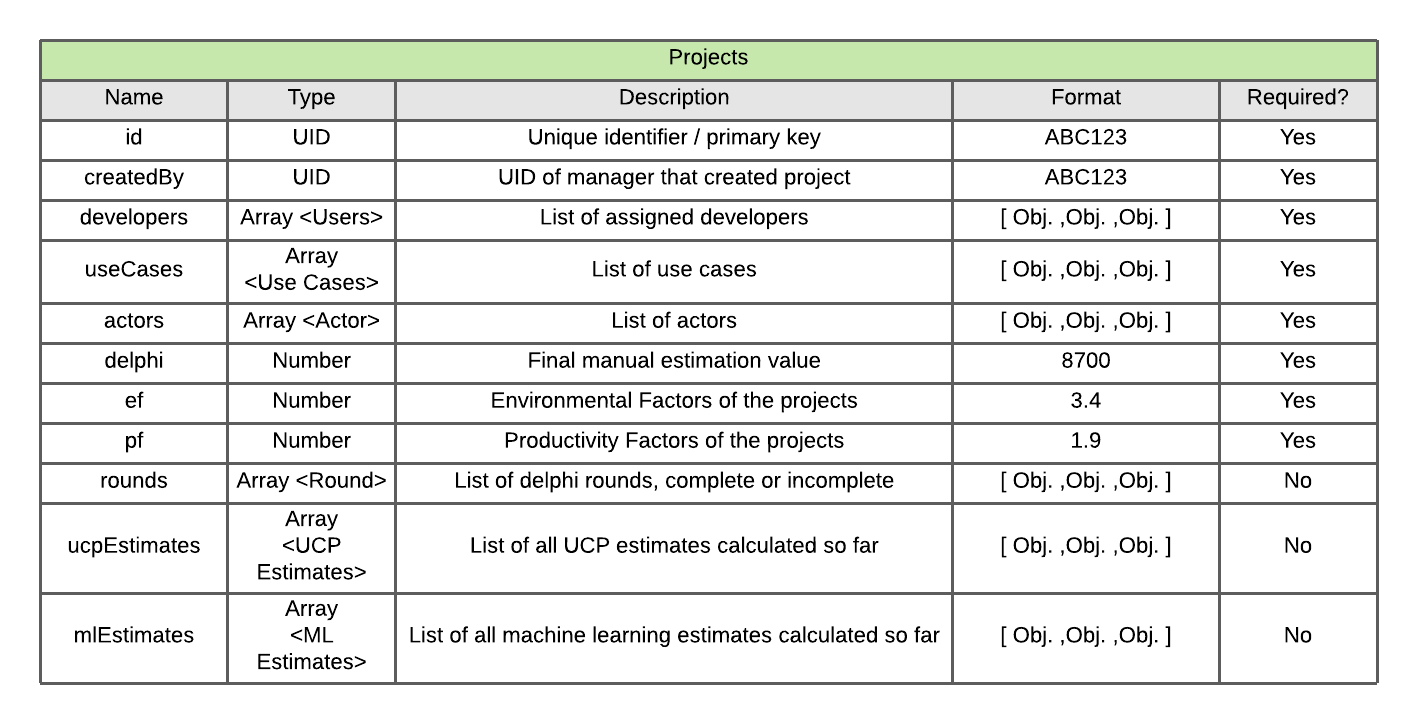
\includegraphics[scale=0.7]{./diagrams/data-dictionary/dd-2.png}
    \label{fig:dd-diag-2}
\end{figure}


\begin{figure}[H]
    \centering
    \caption{Data Dictionary Diagram 3}
    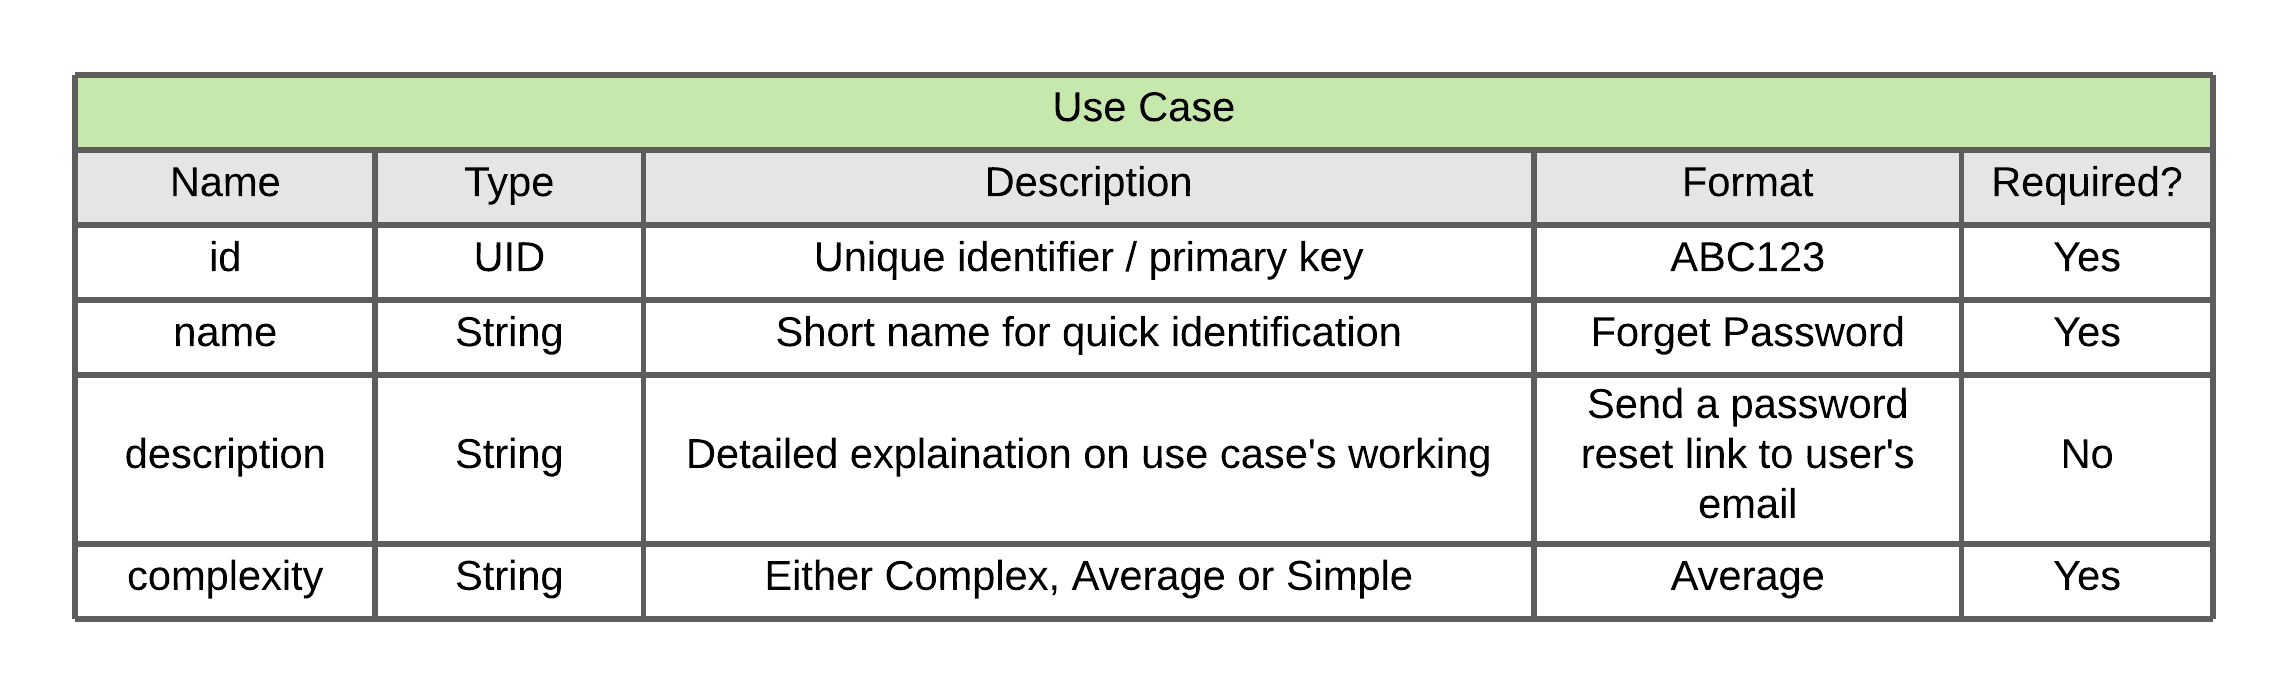
\includegraphics[scale=0.7]{./diagrams/data-dictionary/dd-3.png}
    \label{fig:dd-diag-3}

\end{figure}


\begin{figure}[H]
    \centering
    \caption{Data Dictionary Diagram 4}
    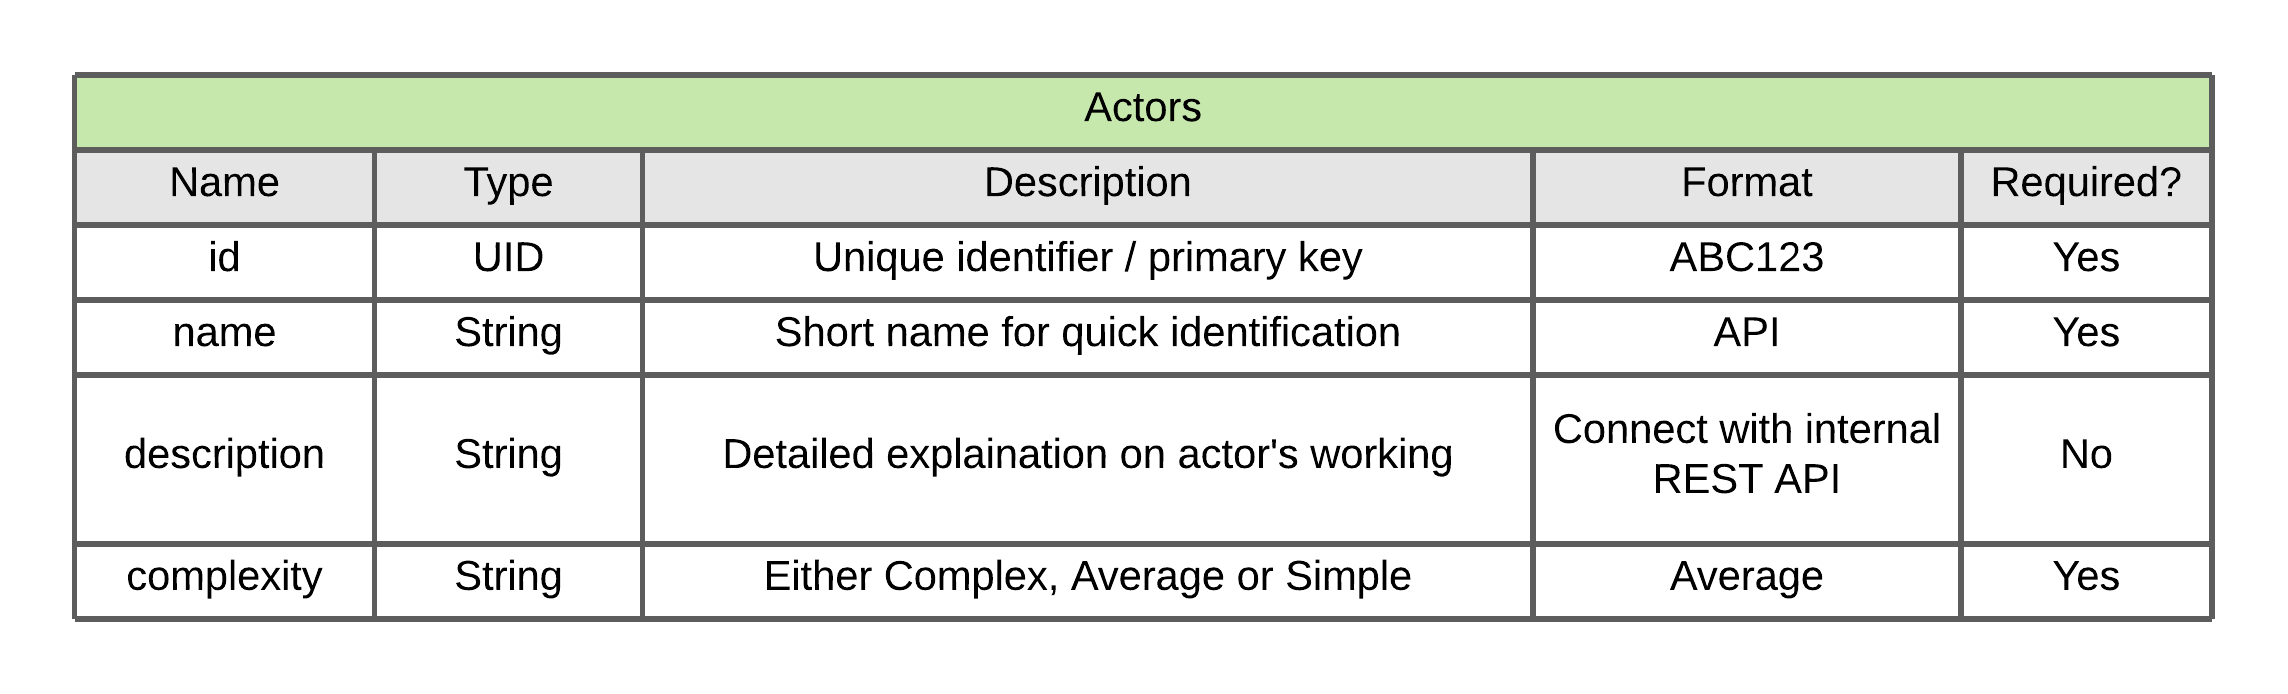
\includegraphics[scale=0.7]{./diagrams/data-dictionary/dd-4.png}
    \label{fig:dd-diag-4}

\end{figure}


\begin{figure}[H]
    \centering
    \caption{Data Dictionary Diagram 5}
    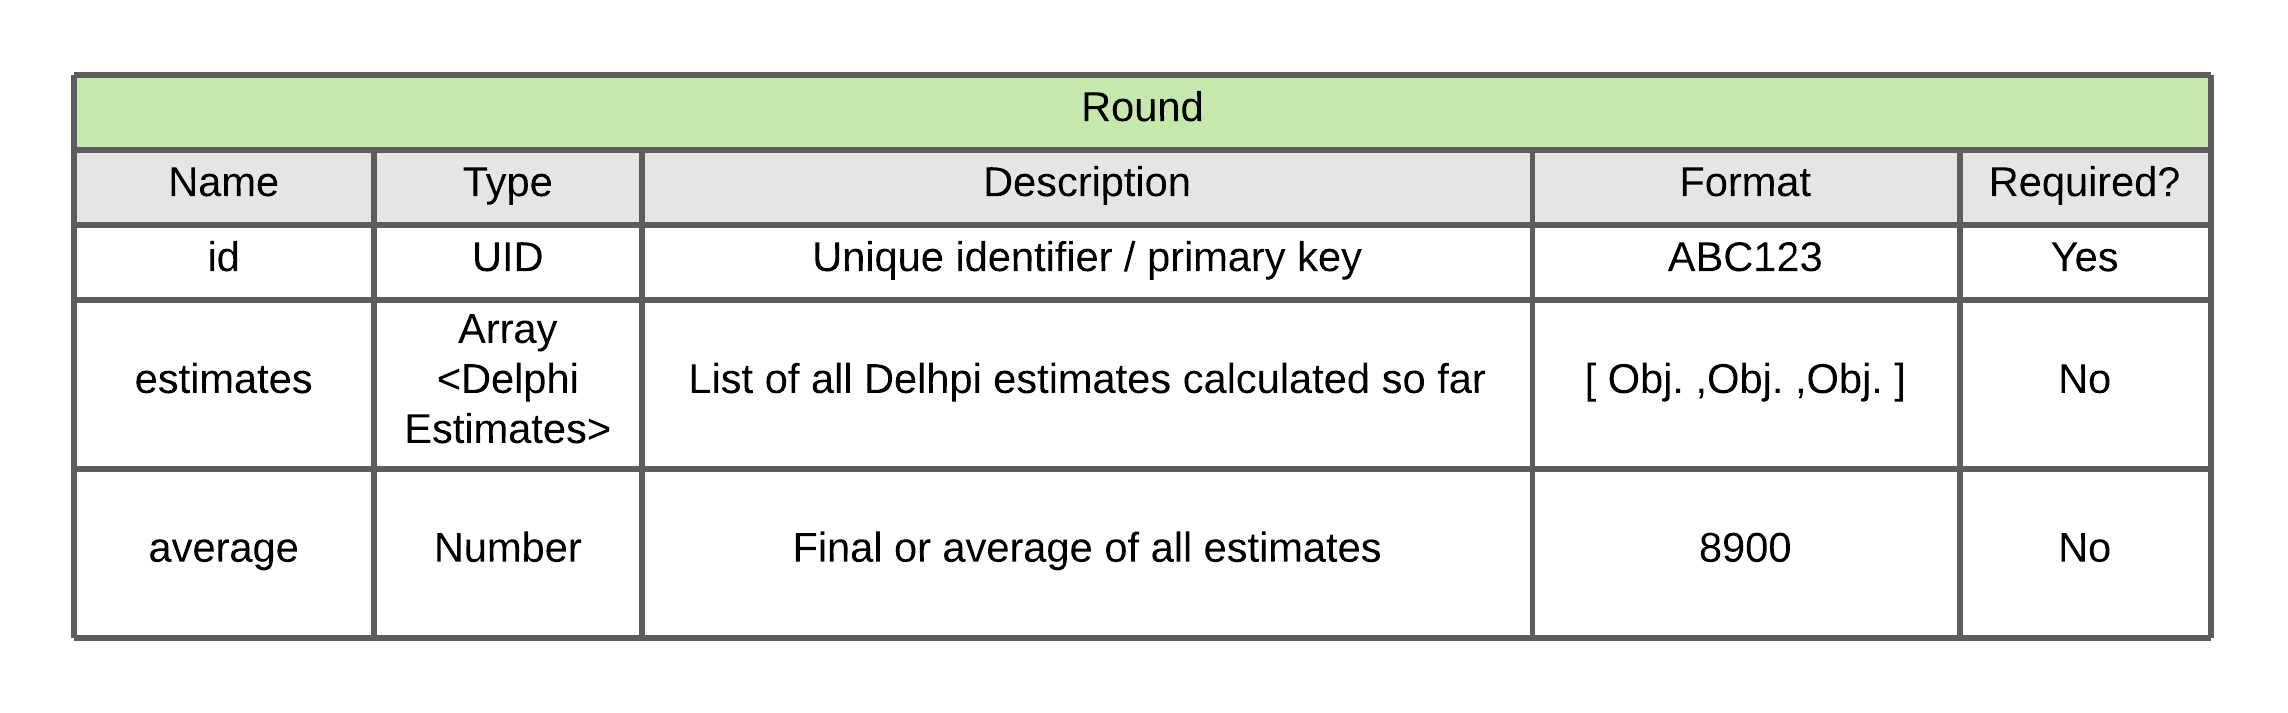
\includegraphics[scale=0.7]{./diagrams/data-dictionary/dd-5.png}
    \label{fig:dd-diag-5}

\end{figure}



\begin{figure}[H]
    \centering
    \caption{Data Dictionary Diagram 6}
    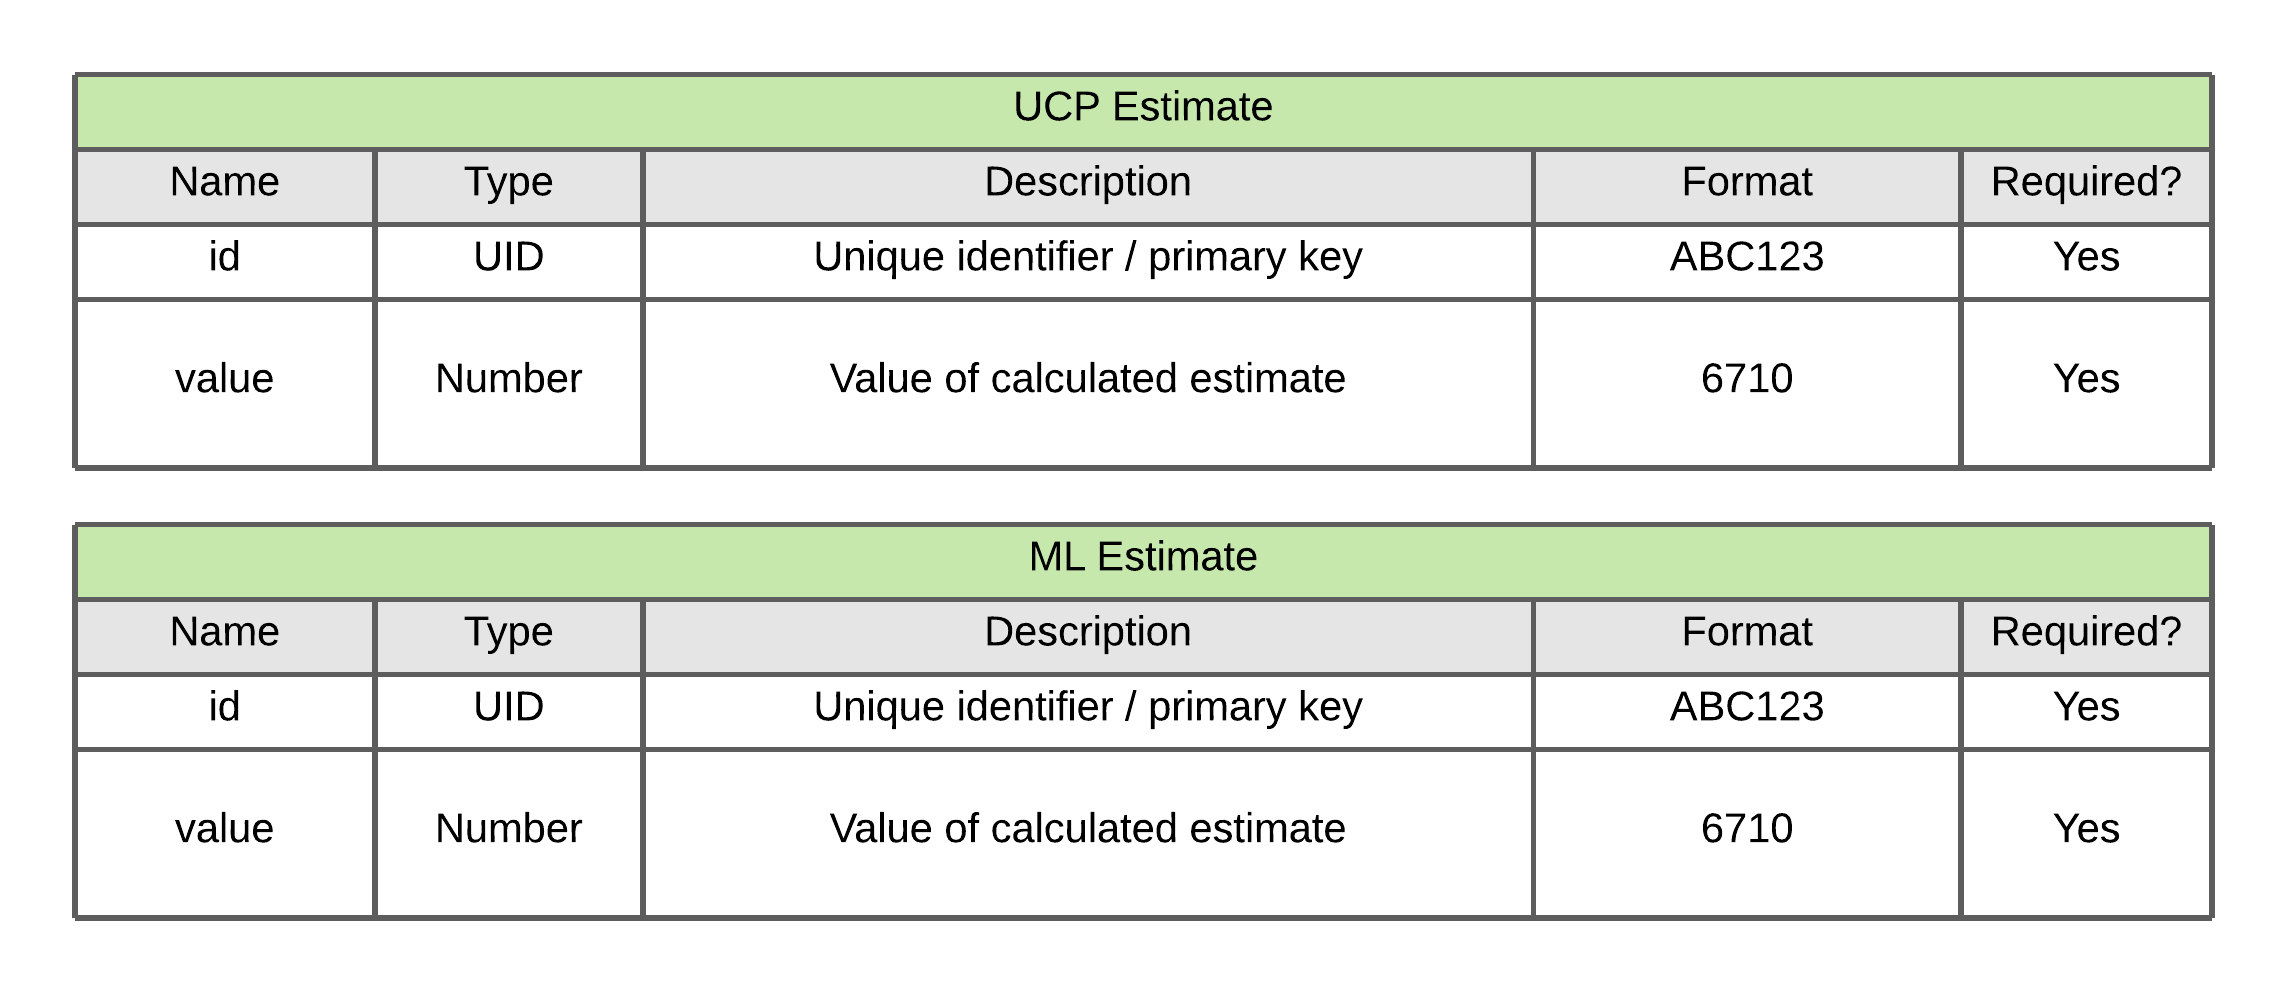
\includegraphics[scale=0.7]{./diagrams/data-dictionary/dd-6.png}
    \label{fig:dd-diag-6}
\end{figure}